\section{Thesis Outline}
\label{sec:intro_outline}
\index{Intro!Thesis Outline}

% ---------------------------------------------------------
% Try to put the figure of the next chapter here
% ---------------------------------------------------------
\begin{figure}[t]
	\centering
	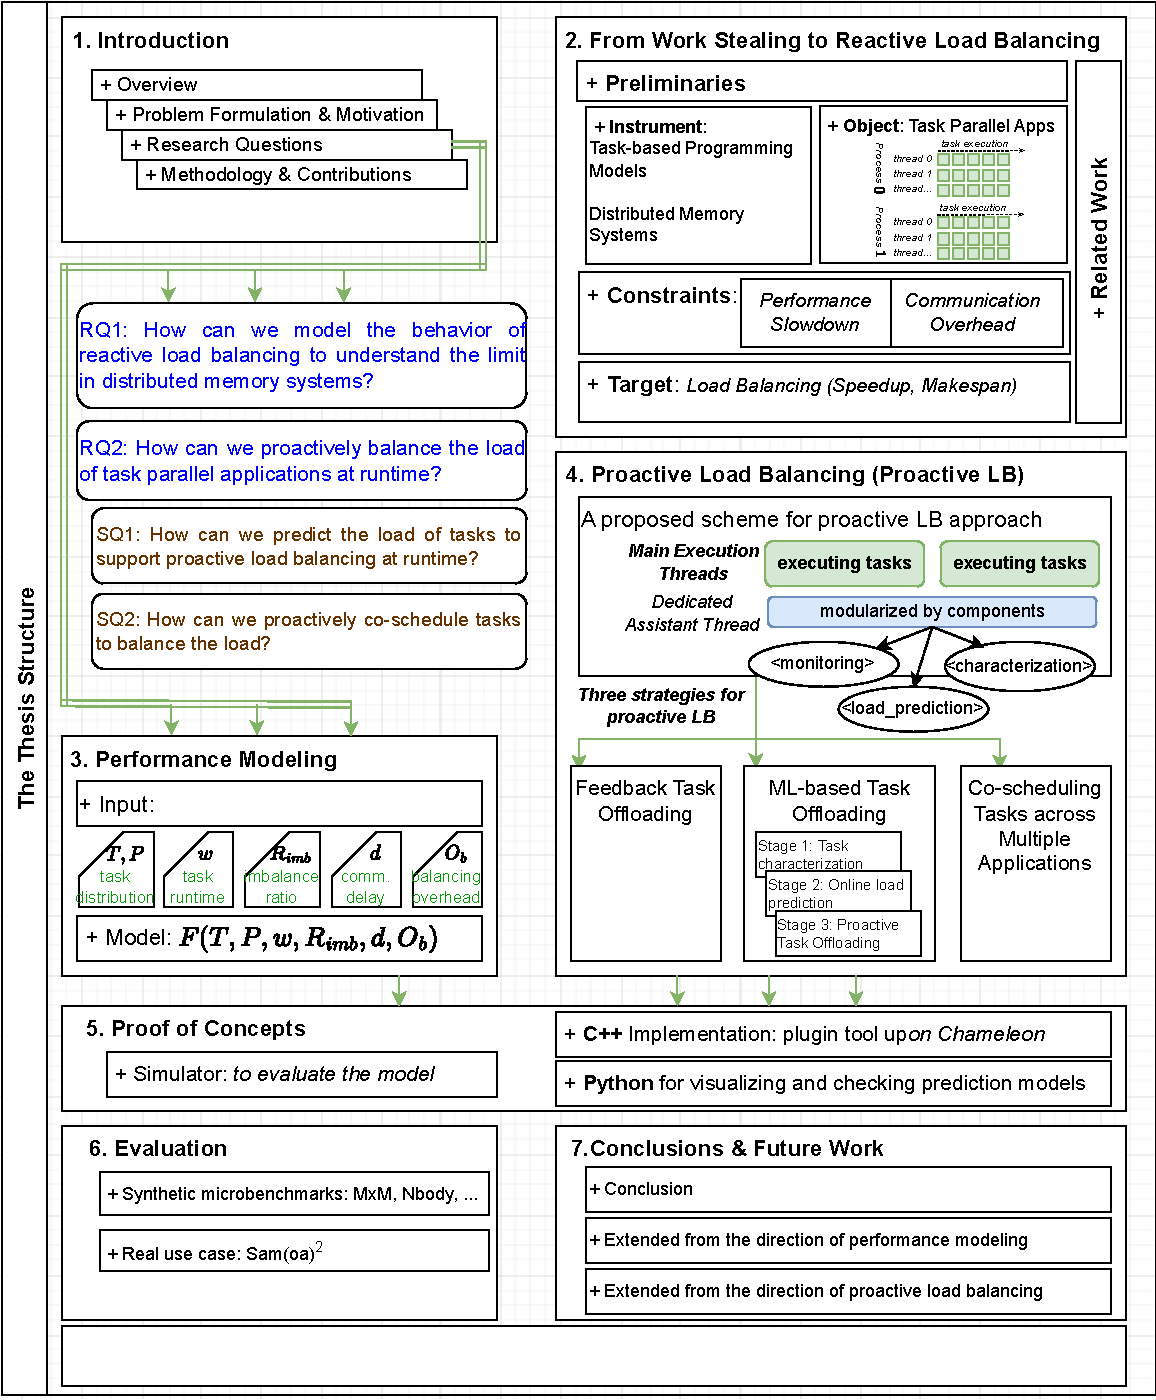
\includegraphics[scale=0.8]{./pictures/introduction/intro_thesis_outline.pdf}
	\caption{The structure of this thesis.}
	\label{fig:intro_outline}
\end{figure}

The structure of this thesis is shown in Figure \ref{fig:intro_outline}. The presented order emphasizes seven parts, where each indicates one chapter. Chapter \ref{ch:Introduction} highlights the overview of our topic and the problem formulation, leading to the motivation and research questions. Additionally, it also introduces the methodology and contribution. Chapter \ref{ch:wstoreactlb} is followed by From Work Stealing to Reactive Load Balancing. We aim to clarify the preliminaries, terminologies, and go through:
\begin{enumerate}
	\item Parallel Programming Models: implies the instruments we use to study dynamic load balancing.
	\item Task-based Parallel Applications: alludes to the object we use to study dynamic load balancing.
	\item Related Work: shows the taxonomy of dynamic load balancing and the state-of-the-art approaches in distributed memory systems. %The evaluation metrics are balancing ratio and speedup in completion time.
\end{enumerate}

Chapter \ref{ch:perfmodel} shows our performance model to analyze the bound of reactive load balancing approaches. The inputs are generalized as a given distribution of $T$ tasks on $P$ processes, the load value of tasks ($w$), imbalance ratio ($R_{imb}$), the overhead of task migration (delay time denoted by $d$) and balancing operation (denoted by $O_{\text{balancing}}$). The model focuses on possibilities when the existing approaches are bounded under the constraints of imbalance level and overhead. \\

Chapter \ref{ch:PADLB} introduces our new proactive load balancing approach. The main idea revolves around how we can predict the tasks' load values at runtime and better guide balancing by proactive task offloading. When we have more knowledge about load values, we can better estimate the number of tasks and potential processes. This approach facilitates two proactive task offloading methods: feedback task offloading and ML-based task offloading. Building upon proactive task offloading, we further introduce an extension of co-scheduling tasks across multiple applications. Our implementation offers a proactive scheme exploiting task-based programming models, where the main threads (execution threads) execute tasks, a dedicated thread ($Tcomm$) performs load prediction and proactive task offloading. For load prediction, $Tcomm$ performs characterizing tasks, training prediction models, and offloading tasks.\\
% Our approach is generally toward one approach which leverages different task offloading methods.

For evaluation, both simulator and reference implementation are used as proof of concepts in Chapter \ref{ch:PoC}. We describe the experiments in Chapter \ref{ch:Evaluation}, where we use synthetic microbenchmarks and a realistic use case of adaptive mesh refinement. Finally, we summarize the conclusions, discuss identified problems, and provide an outlook for future work in Chapter \ref{ch:ConclusionFutureWork}.\\
